\section{Resultados}



Os resultados obtidos estão nas imagens seguintes.

\begin{center}
 	
 	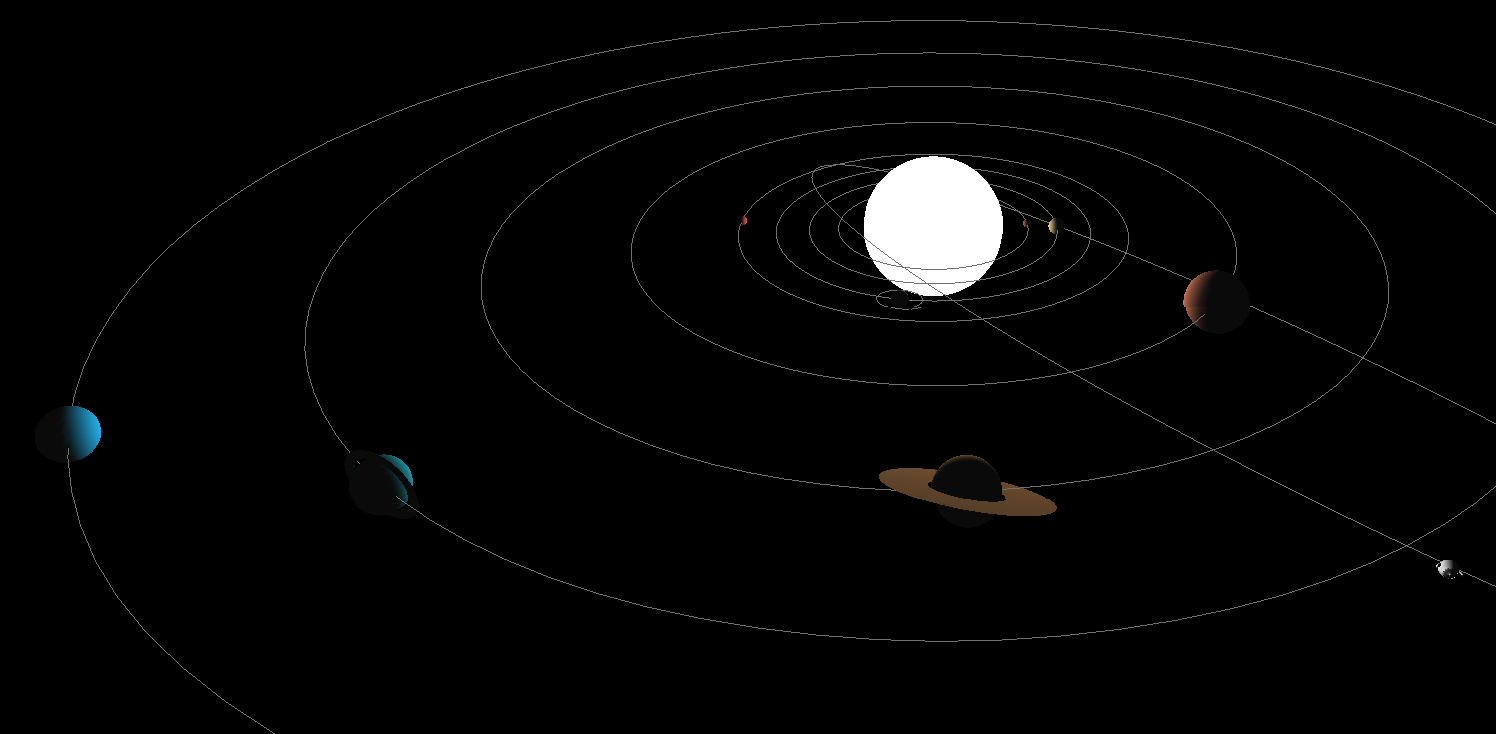
\includegraphics[width=\textwidth,height=\textheight,keepaspectratio]{resources/sistemaRGBA.png}
 	\captionsetup{type=figure, width=0.8\linewidth}
	\caption{\textit{Rendering} do modelo com cores e um luz posicional}
\label{fig:ssec3:tilt} 
\end{center}


\begin{center}
 	
 	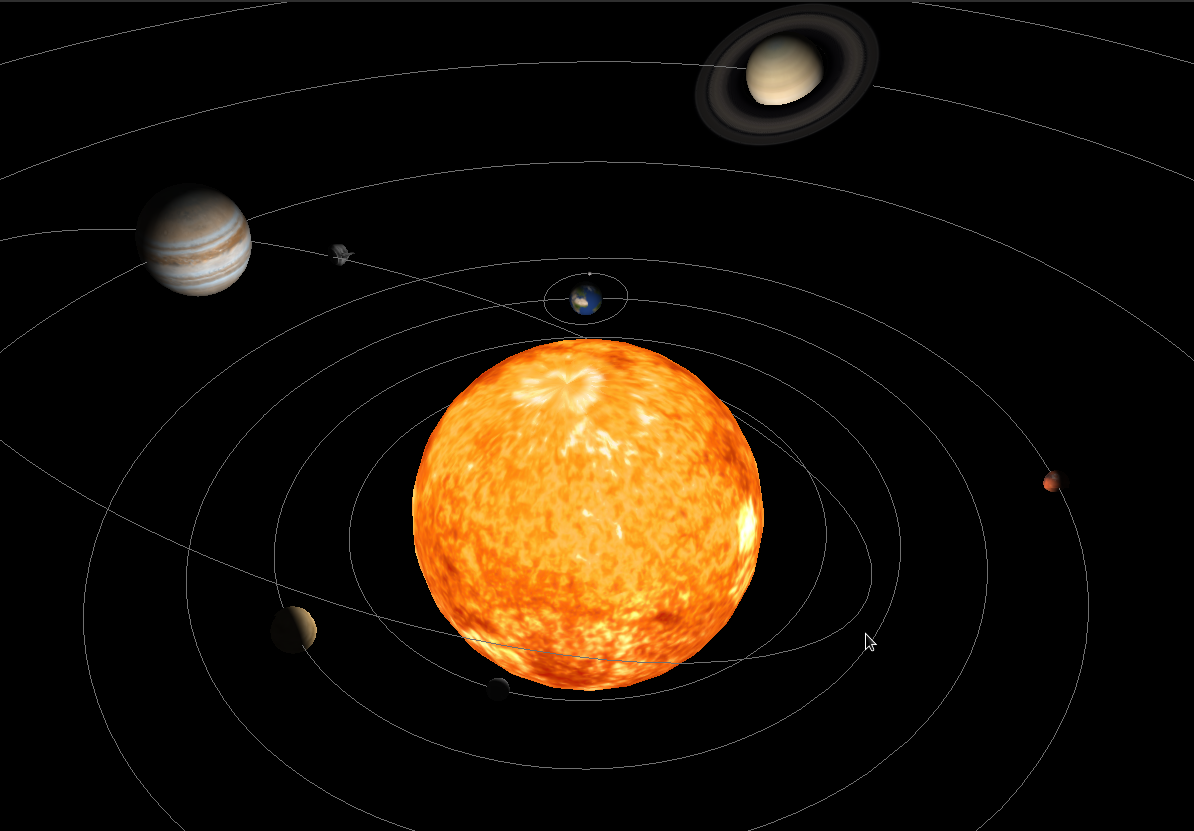
\includegraphics[width=\textwidth,height=\textheight,keepaspectratio]{resources/sistemaSolar.png}
 	\captionsetup{type=figure, width=0.8\linewidth}
	\caption{\textit{Rendering} do modelo com texturas e um luz posicional}
\label{fig:ssec3:tilt} 
\end{center}


A \emph{Figura~\ref{fig:ssec3:modelo}} mostra o modelo com cometa. 

\begin{center}
 	
 	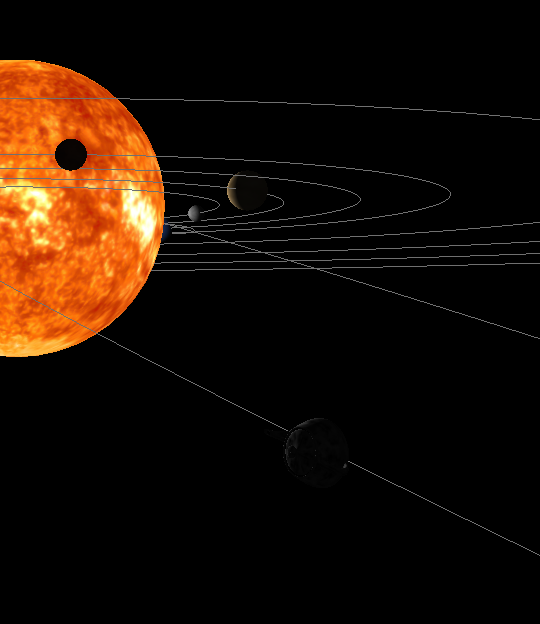
\includegraphics[width=\textwidth,height=\textheight,keepaspectratio]{resources/pormenorCometa.png}
 	\captionsetup{type=figure, width=0.8\linewidth}
	\caption{\textit{Rendering} do modelo com foco no cometa}
\label{fig:ssec3:modelo} 
\end{center}


\begin{center}
 	
 	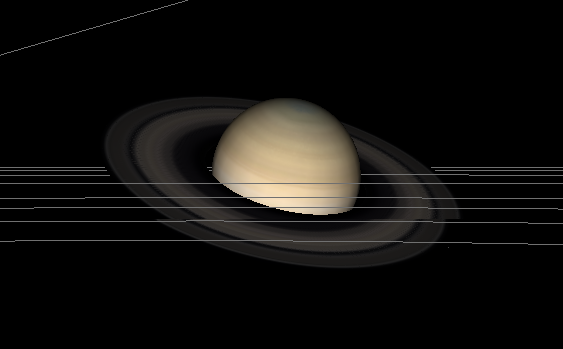
\includegraphics[width=\textwidth,height=\textheight,keepaspectratio]{resources/pormenorSaturno.png}
 	\captionsetup{type=figure, width=0.8\linewidth}
	\caption{\textit{Rendering} do modelo com foco em Saturno}
\label{fig:ssec3:modelo2} 
\end{center}



